\documentclass[aspectratio=169,11pt]{beamer}
\usepackage[utf8]{inputenc}
\usepackage[T1]{fontenc}
\usepackage[italian]{babel}
\usepackage{lmodern}
\usetheme{default}
\setbeamertemplate{navigation symbols}{}
\setbeamertemplate{footline}[frame number]
\graphicspath{{graphs/}}

\begin{document}

\begin{frame}{Petrolio e gas: risposta delle retribuzioni nell'area dell'euro}
  \begin{columns}[T]
    \begin{column}{0.49\textwidth}
      \centering \small Retribuzioni contrattuali\\[0.2em]
      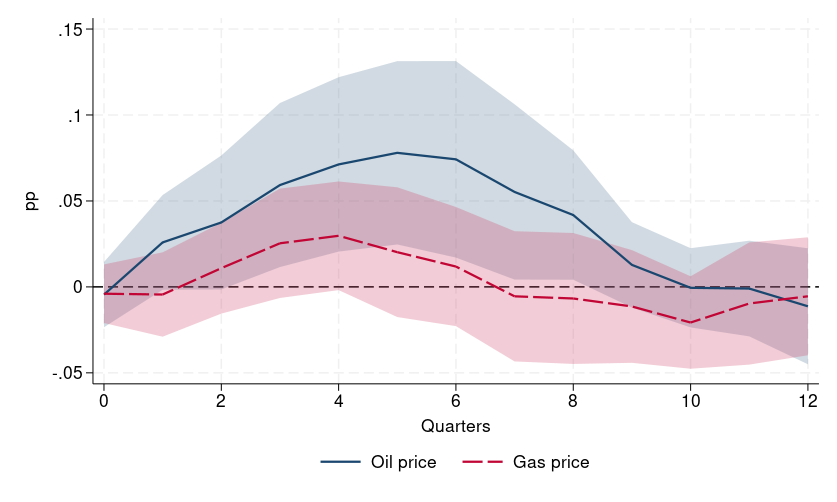
\includegraphics[width=\textwidth]{lp_og_EA_contr.png}
    \end{column}
    \begin{column}{0.49\textwidth}
      \centering \small Retribuzioni lorde per ora lavorata\\[0.2em]
      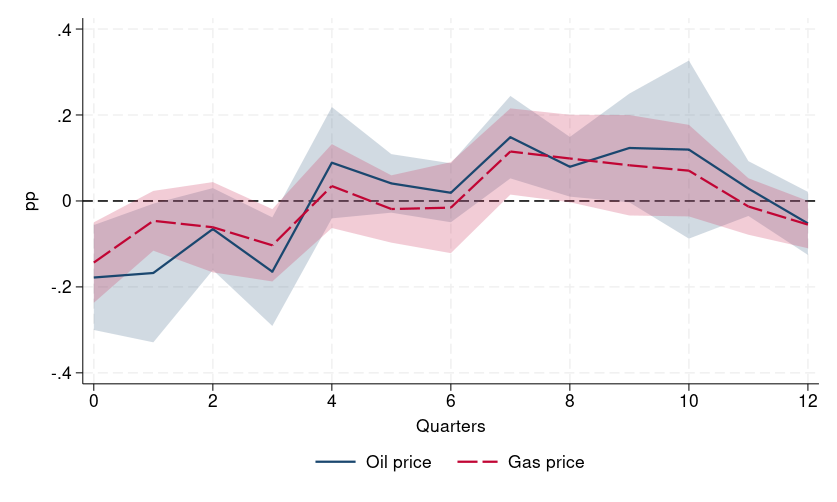
\includegraphics[width=\textwidth]{lp_og_EA_wageH.png}
    \end{column}
  \end{columns}
  \vfill
  {\scriptsize Risposta (punti percentuali) della variazione tendenziale delle retribuzioni
  a un aumento di 10 punti percentuali della variazione tendenziale del prezzo del
  petrolio (blu) e del gas naturale (rosso); bande di confidenza al 90\%. Local
  projections su serie storiche per l'area dell'euro.\par}
\end{frame}

\begin{frame}{Petrolio e gas: area dell'euro e singoli paesi}
  \begin{columns}[T]
    \begin{column}{0.49\textwidth}
      \centering \small Retribuzioni contrattuali\\[0.2em]
      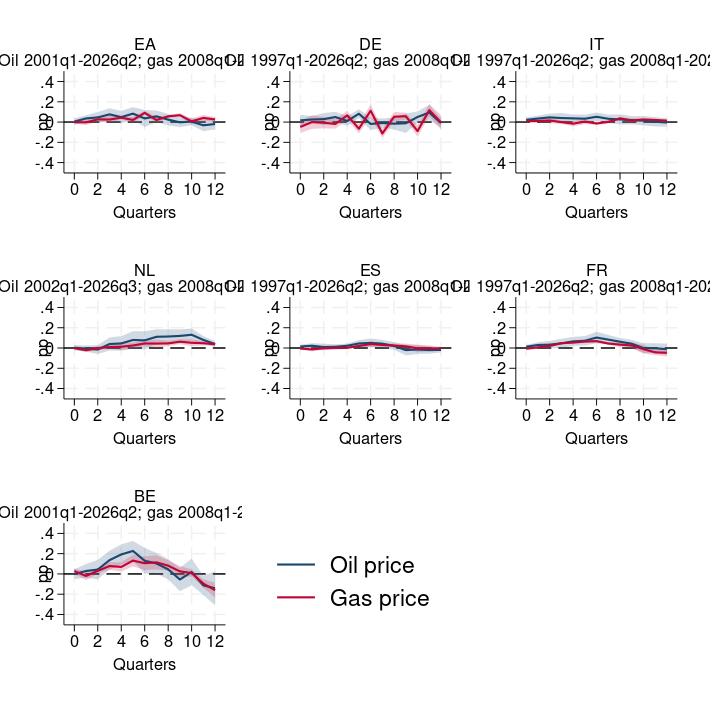
\includegraphics[height=0.66\textheight]{lp_og_ctry_contr_sq.png}
    \end{column}
    \begin{column}{0.49\textwidth}
      \centering \small Retribuzioni lorde per ora lavorata\\[0.2em]
      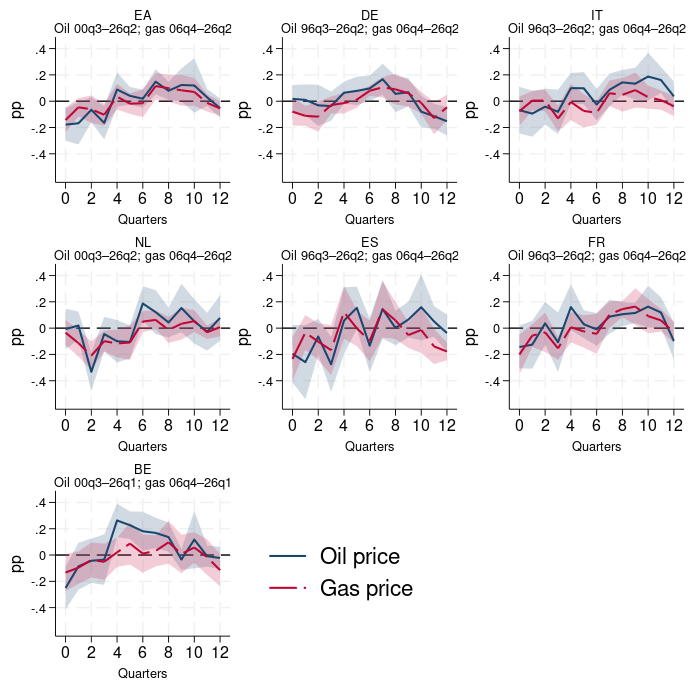
\includegraphics[height=0.66\textheight]{lp_og_ctry_wageH_sq.png}
    \end{column}
  \end{columns}
  \vfill
  {\scriptsize Petrolio in blu, gas naturale in rosso; bande di confidenza al 90\%;
  stessa scala dell'asse verticale nei riquadri di ciascun grafico. Serie storiche per
  l'area dell'euro e per paese.\par}
\end{frame}

\end{document}
